
\documentclass[12pt, twoside]{book}
%%%%%%%% Preamble %%%%%%%%%%%%
\title{Degree project}
\usepackage[utf8]{inputenc} % File coding uses utf8
\usepackage{amsmath} % Extra commands for math
\usepackage{amssymb} % Math symbols 
\usepackage{graphicx} % Include images in LaTeX
\usepackage{color} % Coloring text
\usepackage{enumerate}
\usepackage{float} % Allow you to use [H] specifier to force the position of the images 
\usepackage{capt-of} % Defines a command \captionof for putting a caption to something that’s not a float.
\usepackage{sidecap} % Defines environments called SCfigure and SCtable (analogous to figure and table) to typeset captions sideways
\sidecaptionvpos{figure}{c} % Alignment
\usepackage{caption} % to customize the captions in floating environments like figure and table
\usepackage{commath} % Mathematics typesetting support
\usepackage{cancel} % Place lines through maths formulae
\usepackage{anysize} % to set up document margins
%\marginsize{2cm}{2cm}{2cm}{2cm} % Left, right, up, down
%\usepackage[top=2cm,bottom=4cm,left=1.5cm,right=3cm,asymmetric]{geometry}
\usepackage{appendix} %Extra control of appendices
\usepackage{tocbibind}
\usepackage{anyfontsize}
\newcommand\mymaintitlesize{\fontsize{16pt}{19.2pt}\selectfont}
\newcommand\mysubtitlesize{\fontsize{14pt}{16.8pt}\selectfont}


%EXTRA PACKAGES
\usepackage{multirow}
\usepackage{glossaries}
\usepackage[linesnumbered,ruled,vlined]{algorithm2e}
\usepackage{multirow}
\usepackage{enumerate}
\usepackage{changepage}
\usepackage{alltt}
\usepackage{listings}
\usepackage{lmodern}
\usepackage{gensymb}
\usepackage{caption}
\usepackage{subcaption}
\usepackage{hyperref}
\hypersetup{
    colorlinks,
    citecolor=blue,
    filecolor=black,
    linkcolor=black,
    urlcolor=black
}
\usepackage{setspace}
\setstretch{1.5}
\usepackage{listings}
\usepackage{color}
\lstloadlanguages{C,C++,csh,Java}

\definecolor{red}{rgb}{0.6,0,0} 
\definecolor{blue}{rgb}{0,0,0.6}
\definecolor{green}{rgb}{0,0.8,0}
\definecolor{cyan}{rgb}{0.0,0.6,0.6}

\lstset{
language=csh,
basicstyle=\footnotesize\ttfamily,
numbers=left,
numberstyle=\tiny,
numbersep=5pt,
tabsize=2,
extendedchars=true,
breaklines=true,
frame=b,
stringstyle=\color{blue}\ttfamily,
showspaces=false,
showtabs=false,
xleftmargin=17pt,
framexleftmargin=17pt,
framexrightmargin=5pt,
framexbottommargin=4pt,
commentstyle=\color{green},
morecomment=[l]{//}, %use comment-line-style!
morecomment=[s]{/*}{*/}, %for multiline comments
showstringspaces=false,
morekeywords={ abstract, event, new, struct,
as, explicit, null, switch,
base, extern, object, this,
bool, false, operator, throw,
break, finally, out, true,
byte, fixed, override, try,
case, float, params, typeof,
catch, for, private, uint,
char, foreach, protected, ulong,
checked, goto, public, unchecked,
class, if, readonly, unsafe,
const, implicit, ref, ushort,
continue, in, return, using,
decimal, int, sbyte, virtual,
default, interface, sealed, volatile,
delegate, internal, short, void,
do, is, sizeof, while,
double, lock, stackalloc,
else, long, static,
enum, namespace, string},
keywordstyle=\color{cyan},
identifierstyle=\color{red},
backgroundcolor=\color{white},
}

\usepackage{caption}
\DeclareCaptionFont{white}{\color{white}}
\DeclareCaptionFormat{listing}{\colorbox{blue}{\parbox{\textwidth}{\hspace{15pt}#1#2#3}}}
\captionsetup[lstlisting]{format=listing,labelfont=white,textfont=white, singlelinecheck=false, margin=0pt, font={bf,footnotesize}}

\lstdefinestyle{sharpc}{language=[Sharp]C, frame=lr, rulecolor=\color{blue!80!black}}

% Reset page margins properly for doublesided pages
\setlength{\marginparwidth}{0pt}
\setlength{\marginparsep}{0pt}
\setlength{\oddsidemargin}{0.125in}
\setlength{\evensidemargin}{0.125in}
\setlength{\textwidth}{6.375in}
\raggedbottom


%%% Theorem-like environments %%%%%%%%%%%%%%%%%%%%%%%%%%%%%%%%%%%%%%%%%%%%%%%%%%
%%\usepackage{mathtools}

\newtheorem{theorem}{Theorem}
\newtheorem{corollary}{Corollary}
\newtheorem{lemma}{Lemma}
\newtheorem{proposition}{Proposition}
\newtheorem{conjecture}{Conjecture}
\newtheorem{definition}{Definition}
\newtheorem{remark}{Remark}
\newtheorem{example}{Example}

%%%%%%%%%%%%%%%%%%%%%%%%%%%%%%%%%%%%%%%%%%%%%%%%%%%%%%%%%%%%%%%%%%%%%%%%%%%%%%%%

%%% Put your local definitions here %%%%%%%%%%%%%%%%%%%%%%%%%%%%%%%%%%%%%%%%%%%%
% For example,
\newcommand{\R}{\mathbb{R}}


% Header and Footer
\usepackage{fancyhdr} 
\pagestyle{fancy}
\fancyhf{}
\fancyhead[L]{\footnotesize Universidad Adolfo Ibáñez} 
\fancyhead[R]{\footnotesize Master of Science in Data Science}   
\fancyfoot[R]{\footnotesize Tesis de Magister}  
\fancyfoot[C]{\thepage}  % center
\fancyfoot[L]{\footnotesize Master of Science in Data Science / Universidad Adolfo Ibáñez}  %left
\renewcommand{\footrulewidth}{0.4pt}
\fancypagestyle{firststyle}
{
   \fancyhf{}
}

\usepackage{listings} % To use source code
\definecolor{dkgreen}{rgb}{0,0.6,0} % Color for using code
\definecolor{gray}{rgb}{0.5,0.5,0.5} 
% Language to use
\usepackage[spanish]{babel}
%\renewcommand{\thechapter}{\Roman{chapter}}



\title{Degree project}




\newglossaryentry{stigmergy}
{
        name=stigmergy,
        description={It is an environmental mechanism to regulate the activity of independent actors or agents}
}
 

%%%%%%%% Preamble ends %%%%%%%%%%%%

\begin{document}
\linespread{1.25}
%%%%%%%%%%%%%%%%%%%%%%%%%%%%%%%% Cover Page %%%%%%%%%%%%%%%%%%%%%%%%%%%%%%%%%%%%%%%%%%%

\thispagestyle{firststyle}
\begin{center}
\begin{figure}
    \centering
    %
\includegraphics[scale = 0.63]{images/yachaytech.png}
\end{figure}
{\fontsize{18pt}{21.6pt}\selectfont \textbf{Universidad Adolfo Ibáñez}}\\
\vspace*{0.75cm}
{\mysubtitlesize{\textbf{Master of Science in Data Science}}}\\
\vspace*{1.75cm}
{\mymaintitlesize{\textbf{TÍTULO: XXXXXXX}}\\
\vspace*{0.75cm}
Trabajo de integración curricular presentado como requisito para la obtención del título de XXXXXX}\\
\vspace*{1.75cm}
{\mysubtitlesize{\textbf{Autor/a:}\\
\vspace*{0.5cm}
Apellidos y Nombre\\
\vspace*{0.75cm}
\textbf{Tutor/a:}\\
\vspace*{0.5cm}
MSDS - Sergio Castillo\\
\vspace*{1.75cm}
Santiago, mes y año}}

\end{center}
\pagenumbering{gobble}
\newpage																		
%%%%%%%%%%%%%%%%%%%% Cover page ends %%%%%%%%%%%%%%%%%%%%%%%%%%%%%%%%


\frontmatter

% \chapter*{\centering Autoría}
% \label{chap:autoria}
% 
Yo, \textbf{NOMBRES Y APELLIDOS}, con cédula de identidad XXXXXXXXXX, declaro que las ideas, juicios, valoraciones, interpretaciones, consultas bibliográficas, definiciones y conceptualizaciones expuestas en el presente trabajo; así cómo, los procedimientos y herramientas utilizadas en la investigación, son de absoluta responsabilidad de el/la autor/a del trabajo de integración curricular. Así mismo, me acojo a los reglamentos internos de la Universidad de Investigación de Tecnología Experimental Yachay.

\vspace{0.6cm}

\noindent Urcuquí, mes y año.

\vspace{2.5cm}

\begin{center}
    \rule[0mm]{60mm}{0.1mm} \\
    {Nombres y Apellidos}\\
    CI:
\end{center}

\thispagestyle{empty} % para que no se numere esta pagina	


% \chapter*{\centering Autorización de publicación}
% \label{chap:autorizacion}
% Yo, \textbf{NOMBRES Y APELLIDOS}, con cédula de identidad XXXXXXXXXX, cedo a la Universidad de Investigación de Tecnología Experimental Yachay, los derechos de publicación de la presente obra, sin que deba haber un reconocimiento económico por este concepto. Declaro además que el texto del presente trabajo de titulación no podrá ser cedido a ninguna empresa editorial para su publicación u otros fines, sin contar previamente con la autorización escrita de la Universidad.

\vspace{0.6cm}

\noindent Asimismo, autorizo a la Universidad que realice la digitalización y publicación de este trabajo de integración curricular en el repositorio virtual, de conformidad a lo dispuesto en el Art. 144 de la Ley Orgánica de Educación 

\vspace{0.6cm}

\noindent Urcuquí, mes y año.

\vspace{2.5cm}

\begin{center}
    \rule[0mm]{60mm}{0.1mm} \\
    {Nombres y Apellidos}\\
    CI:
\end{center}

\thispagestyle{empty} % para que no se numere esta pagina

% \chapter{\centering Dedication}
% \label{chap:dedication}
% \begin{center}
	
	The student can use this space, if desired, to write a dedication with a maximum length of one page.
\end{center}
\vspace{8cm}
\begin{flushright}
    Full Name
\end{flushright}

% \chapter{\centering Acknowledgment}
% \label{chap:acknowledgments}
% The student can use this space to show acknowledgemet, if desired. Maximum one page.

\vspace{5cm}
\begin{flushright}
    Full Name
\end{flushright}

% \chapter{\centering Resumen}
% \label{chap:resumen}
% El resumen es una presentación abreviada. Se debe usar una extensión máxima de 250 palabras. Se recomienda que este resumen sea analítico, es decir que sea completo, con información cuantitativa y cualitativa.\\

\noindent \textbf{Palabras Clave}:\\
Al final del resumen se deben usar palabras claves tomadas del texto, las cuales permiten la recuperación de la información, (Mínimo 3 y máximo 7 palabras, preferiblemente use lenguaje técnico-científico). No se deberá usar siglas, ni formulas con caracteres especiales.

% \chapter{\centering Abstract}
% \label{chap:abstract}
% Es el mismo resumen, pero traducido al idioma inglés.\\

\noindent \textbf{Keywords}:\\
Al final del resumen se deben usar palabras claves tomadas del texto, las cuales permiten la recuperación de la información, (Mínimo 3 y máximo 7 palabras, preferiblemente use lenguaje técnico-científico), en idioma inglés. No se deberá usar siglas, ni formulas con caracteres especiales.

% \tableofcontents 
% \printglossaries
% \listoftables
% \listoffigures

%Indice
%\tableofcontents

\mainmatter

\newpage

\chapter{Introducción}
\label{chap:intro}
%---------------------------------------------------------
% \section{Background}

El Reconocimiento de la Actividad Humana\cite{Humanactivityrecognition} (Human Activity Recognition) es un tema que se ha sido objeto de distintos estudios e investigaciones. 
Human Activity Recognition o como se conoce en sus siglas, HAR, se define como la habilidad de interpretar los movimientos o gestos humanos a través de sensores para reconocer la actividad o acción humana.\cite{10.1007/s11390-011-9430-9}

Este campo de investigación es clave dentro del campo de la computación ubicua\cite{10.5555/2832747.2832806}, y a partir de estos estudios se pueden desarrollar herramientas para el desarrollo de las personas en áreas como sistemas de vigilancia\cite{10.1007/s11390-011-9430-9}, la salud\cite{10.1145/3195106.3195157}, interacción humana con computadores\cite{10.1007/s11390-011-9430-9}, y cualquier campo relacionado donde sea aplicable. \newline
Uno de los campos que abre este tipo de investigaciones el de métodos de transporte\cite{Efthymiou2019}. Los métodos de transporte han abierto un campo dentro de la computación ubicua. Debido a la aparición de nuevos dispositivos móviles como smartphones y weareables, se han abierto nuevas oportunidades para la exploración de este tema.


asdasdasdasd


%---------------------------------------------------------

%\section{Problem statement}


%\section{Objectives}

%\subsection{General Objective}



%\subsection{Specific Objectives}


%\section{Justification}


%\chapter{Theoretical Framework}
%\label{chap:theory}
%[Theoretical framework text here]

\begin{figure}[h]
    \centering
    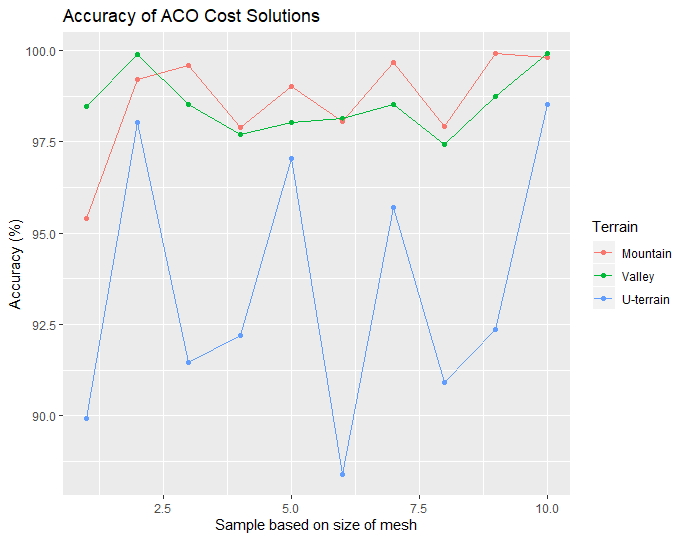
\includegraphics[width=0.7\textwidth]{images/accuracy_example_fig.png}
    \caption{Figure's description.}
     \label{fig:description}
\end{figure}

%\chapter{State of the Art}
%\label{chap:state_of_art}
%[State of the art]

%\chapter{Problem Setting}
%label{chap:problem_setting}
%problem setting

%\chapter{Methodology}
%\label{chap:methods}
%    \section{Phases of Problem Solving}
    
    \subsection{Description of the Problem}
    
    \subsection{Analysis of the Problem}
    
    \subsection{Algorithm Design}
    
    \subsection{Implementation}
    
    \subsection{Testing}

\section{Model Proposal}

\section{Analysis Method}

\section{Experimental Setup}


%\chapter{Results and Discussion}
%\label{chap:results}
%[Your results here]


%\chapter{Discussion}
%\label{chap:results}
%your discussion


%\chapter{Conclusions}
%\label{chap:conclusions}
%[Your conclusions]


\newpage


%%%%%%% Bibliography %%%%%%%%
\bibliographystyle{bst/IEEEtran} 
\bibliography{bib/IEEEreferences} 
%%%%%%% Bibliography %%%%%%%%    

% \appendix  
\newpage
\clearpage % o \cleardoublepage
% \addappheadtotoc 
% \appendixpage 

% \section{Appendix 1. }
[Your appendix]



\end{document}